\documentclass{amsart}
\usepackage{amsmath,amssymb,stmaryrd,tikz}

\newtheorem{prop}{Proposition}

\newcommand{\id}{\mathrm{id}}
\newcommand{\Ob}{\operatorname{Ob}}
\newcommand{\Arr}{\operatorname{Arr}}
\newcommand{\transformto}{\to}
\newcommand{\base}{\mathrm{base}}
\newcommand{\sub}{\mathrel{\triangleleft}}
\newcommand{\subd}{\mathrel{\!\vcenter{\hbox{\larger[-12]$\blacktriangleleft$}}\!}}
\newcommand{\idsub}{\id_{\sub}}
\newcommand{\idsubd}{\id_{\subd}}
\newcommand{\direct}[1]{\overset{#1}{\to}}
\newcommand{\posof}{\in}
\newcommand{\canoniso}{=}

\newcommand{\bundle}[1]{\overset{#1}{\to}}
\newcommand{\pos}[1]{#1(1)}
\newcommand{\posmap}[1]{#1_1}
\newcommand{\shrink}[2][.5]{\scalebox{#1}{$#2$}}


\definecolor{rcol}{RGB}{255,0,0}
\definecolor{gcol}{RGB}{0,150,0}
\definecolor{pcol}{RGB}{170,0,170}
\definecolor{bcol}{RGB}{0,0,255}
\definecolor{ycol}{RGB}{210,130,0}

\tikzset{every picture/.style={scale=.1,baseline}}

\tikzset{vertex/.style={circle,draw,inner sep=1pt,minimum size=6,text=black}}
\tikzset{edge/.style={-stealth}}
\tikzset{label/.style={rectangle,rounded corners,fill=white,inner
sep=1pt,text=black}}

\tikzset{annot/.style={font=\scriptsize}}
\tikzset{dash/.style={dashed,draw opacity=0.5}}
\tikzset{transparent/.style={draw opacity=0.3,fill opacity=0.3}}
\tikzset{small/.style={minimum size=3.5}}
\tikzset{large/.style={minimum size=12}}
\tikzset{huge/.style={minimum size=17}}
\tikzset{huger/.style={minimum size=27}}
\title{Polynomial comonoids and bicomodules}
\begin{document}
\maketitle

\vspace{1.5em}

\iffalse
  A \emph{polynomial}\footnote{The name refers to a correspondence
    between families of sets and sums of powers, illustrated by the
    example
    ${2y^4 + y^2 + y \leftrightarrow
      \{\{\ast,\ast,\ast,\ast\},\{\ast,\ast,\ast,\ast\},\{\ast,\ast\},
      \{\ast\}\}}$.} is an indexed family of sets.

  The indexes of sets are called \emph{positions}, and the members of
  indexed sets are called \emph{directions}.

  We will visualize a polynomial as a collection of corollas.

  % figure

  A corolla is a node with arrows pointing out from it; this denotes a
  position and the directions from it.
\fi

Recall the \emph{substitution product} of polynomials $P$ and $Q$, denoted
$P \sub Q$.

\iffalse
  From polynomials $P$ and $Q$, we can form a new polynomial
  of all the possible two-story trees built by stacking $Q$
  corollas atop a $P$ corolla. This is called the \emph{substitution
    product}, denoted $P \sub Q$.
\fi

\begin{itemize}
\item A position $a$ in $P \sub Q$ consists of a position $a_\base$ in
  $P$ and positions $a_f$ in $Q$ for each direction $f$ from
  $a_\base$.
\item A direction from position $a$ in $P \sub Q$ consists of a
  direction $f$ from $a_\base$ and a direction $g$ from $a_f$.
\end{itemize}
\vspace{.5em}
\begin{center}
  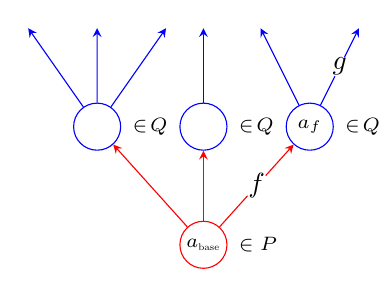
\begin{tikzpicture}
\node [rcol,vertex,huge] (s) at (0, -12) {\scriptsize$a_{\shrink{\base}}$};
\node [bcol,vertex,huge] (m1) at (-13.5,3) {};
\node [bcol,vertex,huge] (m2) at (0,3) {};
\node [bcol,vertex,huge] (m3) at (13.5,3) {\scriptsize$a_f$};
\coordinate (t11) at (-22.25,15.5) {};
\coordinate (t12) at (-13.5,15.5) {};
\coordinate (t13) at (-4.75,15.5) {};
\coordinate (t21) at (0,15.5) {};
\coordinate (t31) at (7.25,15.5) {};
\coordinate (t32) at (19.75,15.5) {};
\draw [rcol,edge] (s) -- (m1);
\draw [rcol,edge] (s) -- (m2);
\draw [rcol,edge] (s) -- node [label] {$f$} (m3);
\draw [bcol,edge] (m1) -- (t11);
\draw [bcol,edge] (m1) -- (t12);
\draw [bcol,edge] (m1) -- (t13);
\draw [bcol,edge] (m2) -- (t21);
\draw [bcol,edge] (m3) -- (t31);
\draw [bcol,edge] (m3) -- node [label] {$g$} (t32);

\node [annot] at (4.5, -12) {\rlap{$\posof P$}};

\node [annot] at (-9, 3) {\rlap{$\posof\!Q$}};
\node [annot] at (4.5, 3) {\rlap{$\posof\!Q$}};
\node [annot] at (18, 3) {\rlap{$\posof\!Q$}};
\end{tikzpicture}

  \qquad
  {\Large$=$}
  \quad
  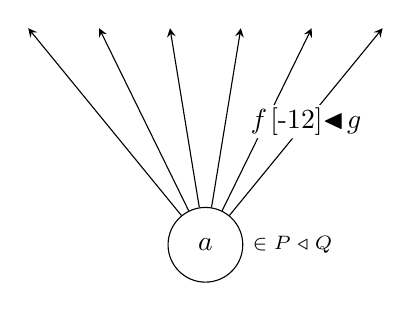
\begin{tikzpicture}
\node [vertex,huger] (s) at (0, -12) {$a$};
\coordinate (t11) at (-22.5,15.5) {};
\coordinate (t12) at (-13.5,15.5) {};
\coordinate (t13) at (-4.5,15.5) {};
\coordinate (t21) at (4.5,15.5) {};
\coordinate (t31) at (13.5,15.5) {};
\coordinate (t32) at (22.5,15.5) {};
\draw [edge] (s) -- (t11);
\draw [edge] (s) -- (t12);
\draw [edge] (s) -- (t13);
\draw [edge] (s) -- (t21);
\draw [edge] (s) -- (t31);
\draw [edge] (s) -- node [label] {$f \subd g$} (t32);

\node [annot] at (6, -12) {\rlap{$\posof P \sub Q$}};
\end{tikzpicture}

\end{center}
\vspace{1em}

We denote such a direction from such a position in a substitution
product by $f \subd g$.\footnote{Be aware there may be other
  directions named $f \subd g$ from other positions in
  $P \sub Q$.} Accordingly, $\idsubd$ will denote the unique direction
from the unique position in the unit for substitution $\idsub$
(a.k.a. the polynomial $y$).\footnote{Given directions $f$,
    $g$, and $h$ respectively belonging to polynomials $P$, $Q$, and
    $R$, the directions of the form $(f \subd g)\subd h$ belonging to
    $(P \sub Q) \sub R$ and the directions of the form
    $f \subd (g \subd h)$ belonging to $P \sub (Q \sub R)$ are
    identified under the relevant monoidal coherence
    isomorphism. Hence brackets can be omitted.

  Similarly, for any direction $f$ belonging to a polynomial $P$, we
  have that $\idsubd \subd f$ and $f \subd \idsubd$ (respectively
  belonging to $\idsub \sub P$ and $P \sub \idsub$) are both
  canonically identified with $f$.}

\iffalse
  Suppose we have polynomials $P$ and $Q$ and the following
  structure relating them.
  \begin{itemize}
  \item A function $\alpha_1$ from the positions of $P$ to the
    positions of $Q$.
  \item For each position $a$ in $P$, a function $\alpha^\sharp_a$ from the
    directions of $\alpha(a)$ back to the directions of $a$.
  \end{itemize}
  This is called a \emph{transformation} from $P$ to $Q$ (written
  $\alpha: P \to Q$).

  We think of this as a way of replacing each corolla from $P$ with a
  a corolla from $Q$.

  % diagram

  The \emph{composite} of transformations $\alpha : P \to Q$ and
  $\beta : Q \to R$, denoted $\alpha \fatsemi \beta : P \to R$,
  is defined by
  \[
    \posmap{(\alpha \fatsemi \beta)}{a} = \posmap{\beta}{\posmap{\alpha}{a}}
    \quad \text{ and } \quad
    \dirmap{(\alpha \fatsemi \beta)}{a}{f} =
    \dirmap{\alpha}{a}{\dirmap{\beta}{\posmap{\alpha}{a}}{f}},
  \] i.e., we do the corolla replacements in order.

  % diagram

  This definition of transformation plays well with the substitution
  product.

  % definition of parallel composition of transformations
\fi

Note the following identity for transformations $\alpha$ and $\beta$
between polynomials.
\[\dirmap{(\alpha \sub \beta)}{a}{f \subd g} = \underbrace{\dirmap{\alpha}{(a_\base)}{f}}_{\backref}
  \subd \dirmap{\beta}{(a_{\backref})}{g}.\] Or in brief, ``we have
$(\alpha \sub \beta)^\sharp(f \subd g) = \alpha^\sharp(f)
\subd\beta^\sharp(g)$ whenever this makes sense.''\footnote{Meaning,
  ${\dirmap{(\alpha \sub \beta)}{a}{f \subd g}}$ exists $\iff$ there are
  $u$ and $v$ such that
  ${\dirmap{\alpha}{u}{f} \subd \dirmap{\beta}{v}{g}}$ actually
  describes a direction from $a$; in this case the two sides are
  equal.
  
  (We are assuming the analogue of this property holds for $\alpha$
  and $\beta$ themselves: if any $\dirmap{\alpha}{u}{f}$ describes a
  direction from $a$, then $\dirmap{\alpha}{a}{f}$ is defined with
  that value --- and likewise for $\beta$. This is trivially so if
  across the domains of $\alpha$ and $\beta$ we use different names
  for different directions.)
  
  \iffalse
    Indeed, the directions from $a$ are of the form $f' \subd g'$,
    where $f'$ is a direction from $a_\base$ and $g'$ is a direction
    from $a_{f'}$. Hence if the expression
    $\dirmap{\alpha}{x}{f} \subd dirmap{\beta}{y}{g}$ is to describe a
    direction from $a$, then $x$ should be $a_\base$, and $y$ should
    be $a_{f'}$.
  \fi
}

\iffalse
  Given a transformation $\alpha$, the map $\alpha_0$ is implicitly
  determined by the domains of the $\alpha^\sharp$
  maps. Moreover, a position in a substitution product is determined
  by the set of names of directions from it (at least, assuming
  the positions in the factor polynomials have this property too), even though
  distinct positions may share certain direction names.

  Hence an equation between horizontal ($\sub$) composites of transformations
  amounts to firstly an identification between domains of the composite
  $\sharp$ maps and secondly their agreement in mapping.

  (We can more generally think of any equality between transformations in
  terms of identification of $\sharp$ maps' domains and their
  agreement in mapping. But this is only interesting when we
  have some reason to think of distinct $\sharp$ domains as sharing
  certain direction names.)

  We can translate arbitrary equalities built from $\sub$
  into equalities built from $\subd$, e.g.
  \[\gamma \fatsemi (\alpha \sub \beta) = \delta \sub \varepsilon
    \iff \gamma^\sharp (\alpha^\sharp \subd \beta^\sharp) =
    \delta^\sharp \subd \varepsilon^\sharp\] for all such
  $\sharp$ maps and values that fit together. Here we may think of the
  equality as indicating agreement about the definedness
  on each potential value of the form $f \subd g$ (i.e. agreement on
  domain), as well as agreement about where each of these values is
  mapped.

  Alternatively, we may think of this fiberwise, such a map being
  completely determined by what subset of values of the form
  $f \subd g$ lies over each individual direction.
\fi

\begin{prop}
  Polynomial comonoids are categories.
\end{prop}
\begin{proof}
  Let $C$ be a polynomial comonoid. Denote counit by $\varepsilon$
  and comultiplication by $\delta$.
  
  \begin{center}
    \input{fig/counit1.tikz}
    \hspace{-.75em}
    $\underset{\varepsilon}{\transformto}$
    \begin{tikzpicture}
\coordinate (s) at (0, -9.5) {};
\coordinate (t1) at (-9,8) {};
\coordinate (t2) at (-3,8) {};
\coordinate (t3) at (3,8) {};
\coordinate (t4) at (9,8) {};
\draw [dash] (s) -- (t1);
\draw [edge] (s) -- node [label] {\scriptsize$\idsubd$} (t2);
\draw [dash] (s) -- (t3);
\draw [dash] (s) -- (t4);
\end{tikzpicture}
    \quad\qquad
    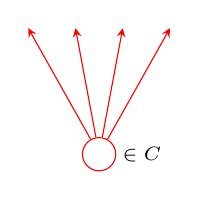
\begin{tikzpicture}
\node [rcol,vertex,large] (s) at (0, -8) {};
\coordinate (t1) at (-9,8) {};
\coordinate (t2) at (-3,8) {};
\coordinate (t3) at (3,8) {};
\coordinate (t4) at (9,8) {};
\draw [rcol,edge] (s) -- (t1);
\draw [rcol,edge] (s) -- (t2);
\draw [rcol,edge] (s) -- (t3);
\draw [rcol,edge] (s) -- (t4);
\node [annot] at (3, -8) {\rlap{$\posof C$}};
\end{tikzpicture}

    \hspace{-.75em}
    $\underset{\delta}{\transformto}$
    \hspace{.5em}
    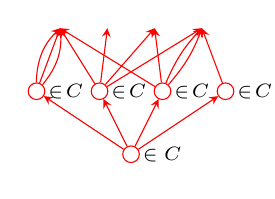
\begin{tikzpicture}
\node [rcol,vertex] (s) at (0, -8) {};
\coordinate (t1) at (-9,8) {};
\coordinate (t2) at (-3,8) {};
\coordinate (t3) at (3,8) {};
\coordinate (t4) at (9,8) {};
\node [rcol,vertex] (m1) at (-12,0) {};
\node [rcol,vertex] (m2) at (-4,0) {};
\node [rcol,vertex] (m3) at (4,0) {};
\node [rcol,vertex] (m4) at (12,0) {};
\draw [rcol,edge] (s) -- (m1);
\draw [rcol,edge] (s) -- (m2);
\draw [rcol,edge] (s) -- (m3);
\draw [rcol,edge] (s) -- (m4);

\draw [rcol,edge] (m1) -- (t1);
\draw [rcol,edge,bend left=22] (m1) to (t1);
\draw [rcol,edge,bend right=22] (m1) to (t1);

\draw [rcol,edge] (m2) -- (t1);
\draw [rcol,edge] (m2) -- (t2);
\draw [rcol,edge] (m2) -- (t3);
\draw [rcol,edge] (m2) -- (t4);

\draw [rcol,edge] (m3) -- (t1);
\draw [rcol,edge] (m3) -- (t3);
\draw [rcol,edge,bend left=10] (m3) to (t4);
\draw [rcol,edge,bend right=10] (m3) to (t4);

\draw [rcol,edge] (m4) -- (t4);

\node [annot] at (1.5, -8) {\rlap{$\posof C$}};

\node [annot] at (-10.5, 0) {\rlap{$\posof\!C$}};
\node [annot] at (-2.5, 0) {\rlap{$\posof\!C$}};
\node [annot] at (5.5, 0) {\rlap{$\posof\!C$}};
\node [annot] at (13.5, 0) {\rlap{$\posof\!C$}};
\end{tikzpicture}

  \end{center}

  \begin{center}
    \begin{tikzpicture}
\coordinate (s) at (0, -8) {};
\coordinate (t1) at (-9,8) {};
\coordinate (t2) at (-3,8) {};
\coordinate (t3) at (3,8) {};
\coordinate (t4) at (9,8) {};
\node [rcol,vertex,transparent] (m1) at (-12,0) {};
\node [rcol,vertex] (m2) at (-4,0) {};
\node [rcol,vertex,transparent] (m3) at (4,0) {};
\node [rcol,vertex,transparent] (m4) at (12,0) {};
\draw [dash] (s) -- (m1);
\draw [edge] (s) -- (m2);
\draw [dash] (s) -- (m3);
\draw [dash] (s) -- (m4);

\draw [rcol,edge,transparent] (m1) -- (t1);
\draw [rcol,edge,bend left=22,transparent] (m1) to (t1);
\draw [rcol,edge,bend right=22,transparent] (m1) to (t1);

\draw [rcol,edge] (m2) -- (t1);
\draw [rcol,edge] (m2) -- (t2);
\draw [rcol,edge] (m2) -- (t3);
\draw [rcol,edge] (m2) -- (t4);

\draw [rcol,edge,transparent] (m3) -- (t1);
\draw [rcol,edge,transparent] (m3) -- (t3);
\draw [rcol,edge,bend left=10,transparent] (m3) to (t4);
\draw [rcol,edge,bend right=10,transparent] (m3) to (t4);

\draw [rcol,edge,transparent] (m4) -- (t4);

\node at (0, -13) {$\delta \fatsemi (\varepsilon \sub \id_C)$};
\end{tikzpicture}

    \quad
    $\canoniso$
    \input{fig/id.tikz}
    $\canoniso$
    \quad
    \begin{tikzpicture}
\node [rcol,vertex] (s) at (0, -8) {};
\coordinate (t1) at (-9,8) {};
\coordinate (t2) at (-3,8) {};
\coordinate (t3) at (3,8) {};
\coordinate (t4) at (9,8) {};
\coordinate (m1) at (-12,0) {};
\coordinate (m2) at (-4,0) {};
\coordinate (m3) at (4,0) {};
\coordinate (m4) at (12,0) {};
\draw [rcol,edge] (s) -- (m1);
\draw [rcol,edge] (s) -- (m2);
\draw [rcol,edge] (s) -- (m3);
\draw [rcol,edge] (s) -- (m4);

\draw [edge] (m1) -- (t1);
\draw [dash,bend left=22] (m1) to (t1);
\draw [dash,bend right=22] (m1) to (t1);

\draw [dash] (m2) -- (t1);
\draw [edge] (m2) -- (t2);
\draw [dash] (m2) -- (t3);
\draw [dash] (m2) -- (t4);

\draw [dash] (m3) -- (t1);
\draw [edge] (m3) -- (t3);
\draw [dash,bend left=10] (m3) to (t4);
\draw [dash,bend right=10] (m3) to (t4);

\draw [edge] (m4) -- (t4);

\node at (0, -13) {$\delta \fatsemi (\id_C \sub \varepsilon)$};
\end{tikzpicture}

  \end{center}

  \begin{center}
    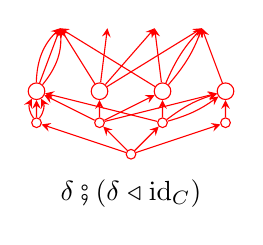
\begin{tikzpicture}
\node [rcol,vertex,small] (s) at (0, -8) {};
\coordinate (t1) at (-9,8) {};
\coordinate (t2) at (-3,8) {};
\coordinate (t3) at (3,8) {};
\coordinate (t4) at (9,8) {};

\node [rcol,vertex,small] (m1_) at (-12,-4) {};
\node [rcol,vertex,small] (m2_) at (-4,-4) {};
\node [rcol,vertex,small] (m3_) at (4,-4) {};
\node [rcol,vertex,small] (m4_) at (12,-4) {};
\draw [rcol,edge] (s) -- (m1_);
\draw [rcol,edge] (s) -- (m2_);
\draw [rcol,edge] (s) -- (m3_);
\draw [rcol,edge] (s) -- (m4_);

\node [rcol,vertex] (m1) at (-12,0) {};
\node [rcol,vertex] (m2) at (-4,0) {};
\node [rcol,vertex] (m3) at (4,0) {};
\node [rcol,vertex] (m4) at (12,0) {};

\draw [rcol,edge] (m1_) -- (m1);
\draw [rcol,edge,bend left=32] (m1_) to (m1);
\draw [rcol,edge,bend right=32] (m1_) to (m1);

\draw [rcol,edge] (m2_) -- (m1);
\draw [rcol,edge] (m2_) -- (m2);
\draw [rcol,edge] (m2_) -- (m3);
\draw [rcol,edge] (m2_) -- (m4);

\draw [rcol,edge] (m3_) -- (m1);
\draw [rcol,edge] (m3_) -- (m3);
\draw [rcol,edge,bend left=10] (m3_) to (m4);
\draw [rcol,edge,bend right=10] (m3_) to (m4);

\draw [rcol,edge] (m4_) -- (m4);


\draw [rcol,edge] (m1) -- (t1);
\draw [rcol,edge,bend left=22] (m1) to (t1);
\draw [rcol,edge,bend right=22] (m1) to (t1);

\draw [rcol,edge] (m2) -- (t1);
\draw [rcol,edge] (m2) -- (t2);
\draw [rcol,edge] (m2) -- (t3);
\draw [rcol,edge] (m2) -- (t4);

\draw [rcol,edge] (m3) -- (t1);
\draw [rcol,edge] (m3) -- (t3);
\draw [rcol,edge,bend left=10] (m3) to (t4);
\draw [rcol,edge,bend right=10] (m3) to (t4);

\draw [rcol,edge] (m4) -- (t4);

\node at (0, -13) {$\delta \fatsemi (\delta \sub \id_C)$};
\end{tikzpicture}
    \quad
    $\canoniso$
    \quad
    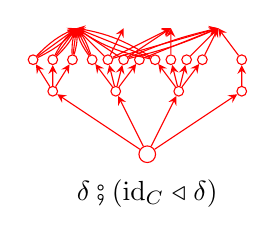
\begin{tikzpicture}
\node [rcol,vertex] (s) at (0, -8) {};
\coordinate (t1) at (-9,8) {};
\coordinate (t2) at (-3,8) {};
\coordinate (t3) at (3,8) {};
\coordinate (t4) at (9,8) {};

\node [rcol,vertex,small] (m1) at (-12,0) {};
\node [rcol,vertex,small] (m2) at (-4,0) {};
\node [rcol,vertex,small] (m3) at (4,0) {};
\node [rcol,vertex,small] (m4) at (12,0) {};
\draw [rcol,edge] (s) -- (m1);
\draw [rcol,edge] (s) -- (m2);
\draw [rcol,edge] (s) -- (m3);
\draw [rcol,edge] (s) -- (m4);

\node [rcol,vertex,small] (m11) at (-14.5,4) {};
\node [rcol,vertex,small] (m12) at (-12,4) {};
\node [rcol,vertex,small] (m13) at (-9.5,4) {};
\node [rcol,vertex,small] (m21) at (-7,4) {};
\node [rcol,vertex,small] (m22) at (-5,4) {};
\node [rcol,vertex,small] (m23) at (-3,4) {};
\node [rcol,vertex,small] (m24) at (-1,4) {};
\node [rcol,vertex,small] (m31) at (1,4) {};
\node [rcol,vertex,small] (m32) at (3,4) {};
\node [rcol,vertex,small] (m33) at (5,4) {};
\node [rcol,vertex,small] (m34) at (7,4) {};
\node [rcol,vertex,small] (m41) at (12,4) {};

\draw [rcol,edge] (m1) -- (m11);
\draw [rcol,edge] (m1) -- (m12);
\draw [rcol,edge] (m1) -- (m13);
\draw [rcol,edge] (m2) -- (m21);
\draw [rcol,edge] (m2) -- (m22);
\draw [rcol,edge] (m2) -- (m23);
\draw [rcol,edge] (m2) -- (m24);
\draw [rcol,edge] (m3) -- (m31);
\draw [rcol,edge] (m3) -- (m32);
\draw [rcol,edge] (m3) -- (m33);
\draw [rcol,edge] (m3) -- (m34);
\draw [rcol,edge] (m4) -- (m41);


\draw [rcol,edge] (m11) -- (t1);
\draw [rcol,edge,bend left=11] (m11) to (t1);
\draw [rcol,edge,bend right=11] (m11) to (t1);

\draw [rcol,edge] (m12) -- (t1);
\draw [rcol,edge,bend left=11] (m12) to (t1);
\draw [rcol,edge,bend right=11] (m12) to (t1);

\draw [rcol,edge] (m13) -- (t1);
\draw [rcol,edge,bend left=11] (m13) to (t1);
\draw [rcol,edge,bend right=11] (m13) to (t1);


\draw [rcol,edge] (m21) -- (t1);
\draw [rcol,edge,bend left=11] (m21) to (t1);
\draw [rcol,edge,bend right=11] (m21) to (t1);

\draw [rcol,edge] (m22) -- (t1);
\draw [rcol,edge] (m22) -- (t2);
\draw [rcol,edge] (m22) -- (t3);
\draw [rcol,edge] (m22) -- (t4);

\draw [rcol,edge] (m23) -- (t1);
\draw [rcol,edge] (m23) -- (t3);
\draw [rcol,edge,bend left=5] (m23) to (t4);
\draw [rcol,edge,bend right=5] (m23) to (t4);

\draw [rcol,edge] (m24) -- (t4);


\draw [rcol,edge] (m31) -- (t1);
\draw [rcol,edge,bend left=11] (m31) to (t1);
\draw [rcol,edge,bend right=11] (m31) to (t1);

\draw [rcol,edge] (m32) -- (t3);

\draw [rcol,edge] (m33) -- (t4);

\draw [rcol,edge] (m34) -- (t4);


\draw [rcol,edge] (m41) -- (t4);

\node at (0, -13) {$\delta \fatsemi (\id_C \sub \delta)$};
\end{tikzpicture}

  \end{center}

  Observe first that the right identity law forces $(\posmap{\delta}{a})_\base = a$
  for all $a \in \pos{C}$.
  Therefore the expression $(\posmap{\delta}{a})_f$ for $f \in C[a]$ has a
  well-defined meaning.

  We gather the data for a category $\cat{C}$.
  \begin{itemize}
  \item The set of objects $\Ob(\cat{C})$ is $\pos{C}$, i.e., the set
    of positions in $C$.
  \item The set of arrows $\Arr(\cat{C})$ is
    $\sum_{a \in \pos{C}}C[a]$, i.e., the set of all directions in $C$.
  \item The source map $s$ sends each $f \in C[a]$ to $a$. (Hence the
    polynomial $C$ is described by the bundle
    $\Arr(\cat{C}) \bundle{s} \Ob(\cat{C})$.)
  \item The target map $t$ sends each $f \in C[a]$ to $(\posmap{\delta}{a})_f$.
  \item The identity map $e$ sends each $a \in \pos{C}$ to
    $\dirmap{\varepsilon}{a}{\idsubd}$.
  \item The composition map $m$ sends each pair of compatible
    arrows ${f \in C[a]}, {g \in C[t(f)]}$ to $\dirmap{\delta}{a}{f \subd g}$.
  \end{itemize}

  Next, observe that if we have such prerequisite data (not laws) for
  a category, subject to just the law $s(e(a)) = a$, then we find that
  further imposing the left identity law $m(e(s(f)), f) = f$
  (requiring that both sides are defined whenever one is)
  automatically forces the law $t(e(a)) = a$ to hold.\footnote{We have
    $m(e(s(e(a))), e(a)) = e(a)$, since the right side is defined. The
    left side reduces to $m(e(a)), e(a))$. This expression only makes
    sense if $t(e(a)) = s(e(a))$, which is $a$.}  Similarly, if we
  have the law $s(m(f,g))=s(f)$ as well as $t(e(a)) = a$, then the
  associativity law $m(m(f,g),h) = m(f,m(g,h))$ forces
  $t(m(f,g)) = t(g)$.\footnote{Given that $f$ and $g$ are composable,
    we have $m(m(f,g),e(t(g))) = m(f,m(g,e(t(g))))$, since the right
    side is defined. The left side only makes sense if
    $t(f,g) = s(e(t(g)))$, which is $t(g)$.}

  We verify the data from above satisfy the laws of a category.
  \begin{itemize}
  \item The law $s(e(a)) = a$ is true by construction; $e(a)$ is a
    direction from the position $a$.
  \item The law $s(m(f, g)) = s(f)$ is true by construction; $m(f, g)$
    is a direction from the position $s(f)$.
  \item The left identity law $m(e(s(f)), f) = f$ is directly
    expressed by the comonoid left identity law, which identifies
    ${\delta^\sharp(\varepsilon^\sharp(\idsubd) \subd f)}$ with $f$.
  \item The right identity law $m(f, e(t(f))) = f$ is directly
    expressed by the comonoid right identity law, which identifies
    ${\delta^\sharp(f \subd \varepsilon^\sharp(\idsubd))}$ with $f$.
  \item The associativity law $m(m(f, g) h) = m(f, m(g, h))$ is
    directly expressed by the comonoid associativity law, which
    identifies ${\delta^\sharp(\delta^\sharp(f \subd g) \subd h)}$ with
    ${\delta^\sharp(f \subd \delta^\sharp(g \subd h))}$.
  \item The law $t(e(a)) = a$ is forced to hold (due to the comonoid
    left identity law).
  \item The law $t(m(f, g)) = t(g)$ is forced to hold (due to the
    comonoid associativity law).
  \end{itemize}

  Conversely, let $\cat{C}$ be a category. We immediately obtain the
  bundle ${\Arr(\cat{C})\bundle{s}\Ob(\cat{C})}$. Let $C$ denote
  the polynomial described by this bundle (the ``outfacing polynomial''
  of $\cat{C}$); we exhibit a comonoid struture on $C$.
  \begin{itemize}
  \item The counit $\varepsilon$ singles out the identity in each
    object's set of outfacing maps.
  \item The comultiplication $\delta$ endows each object $a$ with
    the map $\delta^\sharp_a$ sending $f \subd g$ to $f \fatsemi g$
    for all arrows of the form $f: a \to b$, $g: b \to c$ (through
    which the map $\delta_0$ is implicit).
  \end{itemize}

  The above processes of translation between the prerequisite data
  (not laws) for a category subject to just $s(e(a)) = a$ and
  $s(m(f, g)) = g$, and the prerequisite data (not laws) of a
  polynomial comonoid subject to just
  $(\posmap{\delta}{a})_\base = a$, are inverse by
  construction. Moreover, we saw earlier that the identity and
  associativity category laws, in this context, directly translate
  to the identity and associativity comonoid laws.
\end{proof}

\begin{prop}
  A polynomial right comodule amounts to a family of copresheaves.
\end{prop}
\begin{proof}
  Let $D$ be a polynomial comonoid and let $M$ be a right comodule on
  $D$. Denote right comodule comultiplication by $\rho$.

  \begin{center}
    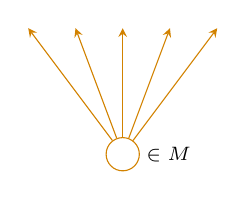
\begin{tikzpicture}
\node [ycol,vertex,large] (s) at (0, -8) {};
\coordinate (t1) at (-12,8) {};
\coordinate (t2) at (-6,8) {};
\coordinate (t3) at (0,8) {};
\coordinate (t4) at (6,8) {};
\coordinate (t5) at (12,8) {};
\draw [ycol,edge] (s) -- (t1);
\draw [ycol,edge] (s) -- (t2);
\draw [ycol,edge] (s) -- (t3);
\draw [ycol,edge] (s) -- (t4);
\draw [ycol,edge] (s) -- (t5);
\node [annot] at (3, -8) {\rlap{$\posof M$}};
\end{tikzpicture}

    \hspace{-.75em}
    $\underset{\rho}{\transformto}$
    \hspace{.5em}
    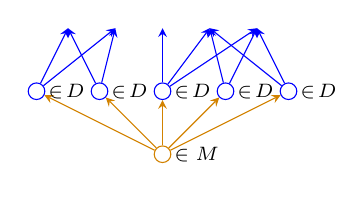
\begin{tikzpicture}
\node [ycol,vertex] (s) at (0, -8) {};
\coordinate (t1) at (-12,8) {};
\coordinate (t2) at (-6,8) {};
\coordinate (t3) at (-0,8) {};
\coordinate (t4) at (6,8) {};
\coordinate (t5) at (12,8) {};
\node [bcol,vertex] (m1) at (-16,0) {};
\node [bcol,vertex] (m2) at (-8,0) {};
\node [bcol,vertex] (m3) at (0,0) {};
\node [bcol,vertex] (m4) at (8,0) {};
\node [bcol,vertex] (m5) at (16,0) {};
\draw [ycol,edge] (s) -- (m1);
\draw [ycol,edge] (s) -- (m2);
\draw [ycol,edge] (s) -- (m3);
\draw [ycol,edge] (s) -- (m4);
\draw [ycol,edge] (s) -- (m5);

\draw [bcol,edge] (m1) -- (t1);
\draw [bcol,edge] (m1) -- (t2);

\draw [bcol,edge] (m2) -- (t1);
\draw [bcol,edge] (m2) -- (t2);

\draw [bcol,edge] (m3) -- (t3);
\draw [bcol,edge] (m3) -- (t4);
\draw [bcol,edge] (m3) -- (t5);

\draw [bcol,edge] (m4) -- (t4);
\draw [bcol,edge] (m4) -- (t5);

\draw [bcol,edge] (m5) -- (t4);
\draw [bcol,edge] (m5) -- (t5);

\node [annot] at (1.5, -8) {\rlap{$\posof M$}};

\node [annot] at (-14.5, 0) {\rlap{$\posof\!D$}};
\node [annot] at (-6.5, 0) {\rlap{$\posof\!D$}};
\node [annot] at (1.5, 0) {\rlap{$\posof\!D$}};
\node [annot] at (9.5, 0) {\rlap{$\posof\!D$}};
\node [annot] at (17.5, 0) {\rlap{$\posof\!D$}};
\end{tikzpicture}

  \end{center}

  \begin{center}
    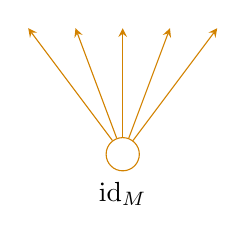
\begin{tikzpicture}
\node [ycol,vertex,large] (s) at (0, -8) {};
\coordinate (t1) at (-12,8) {};
\coordinate (t2) at (-6,8) {};
\coordinate (t3) at (0,8) {};
\coordinate (t4) at (6,8) {};
\coordinate (t5) at (12,8) {};
\draw [ycol,edge] (s) -- (t1);
\draw [ycol,edge] (s) -- (t2);
\draw [ycol,edge] (s) -- (t3);
\draw [ycol,edge] (s) -- (t4);
\draw [ycol,edge] (s) -- (t5);

\node at (0, -13) {$\id_M$};
\end{tikzpicture}

    $\canoniso$
    \quad
    \begin{tikzpicture}
\node [ycol,vertex] (s) at (0, -8) {};
\coordinate (t1) at (-12,8) {};
\coordinate (t2) at (-6,8) {};
\coordinate (t3) at (0,8) {};
\coordinate (t4) at (6,8) {};
\coordinate (t5) at (12,8) {};

\coordinate (m1) at (-16,0) {};
\coordinate (m2) at (-8,0) {};
\coordinate (m3) at (0,0) {};
\coordinate (m4) at (8,0) {};
\coordinate (m5) at (16,0) {};

\draw [ycol,edge] (s) -- (m1);
\draw [ycol,edge] (s) -- (m2);
\draw [ycol,edge] (s) -- (m3);
\draw [ycol,edge] (s) -- (m4);
\draw [ycol,edge] (s) -- (m5);

\draw [edge] (m1) -- (t1);
\draw [dash] (m1) -- (t2);

\draw [dash] (m2) -- (t1);
\draw [edge] (m2) -- (t2);

\draw [edge] (m3) -- (t3);
\draw [dash] (m3) -- (t4);
\draw [dash] (m3) -- (t5);

\draw [edge] (m4) -- (t4);
\draw [dash] (m4) -- (t5);

\draw [dash] (m5) -- (t4);
\draw [edge] (m5) -- (t5);

\node at (0, -13) {$\rho \fatsemi (\id_M \sub \varepsilon)$};
\end{tikzpicture}

  \end{center}

  \begin{center}
    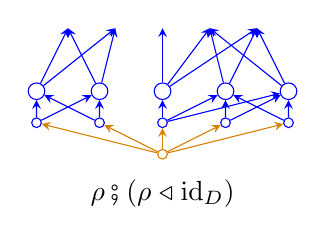
\begin{tikzpicture}
\node [ycol,vertex,small] (s) at (0, -8) {};
\coordinate (t1) at (-12,8) {};
\coordinate (t2) at (-6,8) {};
\coordinate (t3) at (-0,8) {};
\coordinate (t4) at (6,8) {};
\coordinate (t5) at (12,8) {};

\node [bcol,vertex,small] (m1) at (-16,-4) {};
\node [bcol,vertex,small] (m2) at (-8,-4) {};
\node [bcol,vertex,small] (m3) at (0,-4) {};
\node [bcol,vertex,small] (m4) at (8,-4) {};
\node [bcol,vertex,small] (m5) at (16,-4) {};

\node [bcol,vertex] (m1_) at (-16,0) {};
\node [bcol,vertex] (m2_) at (-8,0) {};
\node [bcol,vertex] (m3_) at (0,0) {};
\node [bcol,vertex] (m4_) at (8,0) {};
\node [bcol,vertex] (m5_) at (16,0) {};

\draw [ycol,edge] (s) -- (m1);
\draw [ycol,edge] (s) -- (m2);
\draw [ycol,edge] (s) -- (m3);
\draw [ycol,edge] (s) -- (m4);
\draw [ycol,edge] (s) -- (m5);

\draw [bcol,edge] (m1) -- (m1_);
\draw [bcol,edge] (m1) -- (m2_);

\draw [bcol,edge] (m2) -- (m1_);
\draw [bcol,edge] (m2) -- (m2_);

\draw [bcol,edge] (m3) -- (m3_);
\draw [bcol,edge] (m3) -- (m4_);
\draw [bcol,edge] (m3) -- (m5_);

\draw [bcol,edge] (m4) -- (m4_);
\draw [bcol,edge] (m4) -- (m5_);

\draw [bcol,edge] (m5) -- (m4_);
\draw [bcol,edge] (m5) -- (m5_);

\draw [bcol,edge] (m1_) -- (t1);
\draw [bcol,edge] (m1_) -- (t2);

\draw [bcol,edge] (m2_) -- (t1);
\draw [bcol,edge] (m2_) -- (t2);

\draw [bcol,edge] (m3_) -- (t3);
\draw [bcol,edge] (m3_) -- (t4);
\draw [bcol,edge] (m3_) -- (t5);

\draw [bcol,edge] (m4_) -- (t4);
\draw [bcol,edge] (m4_) -- (t5);

\draw [bcol,edge] (m5_) -- (t4);
\draw [bcol,edge] (m5_) -- (t5);


\node at (0, -13) {$\rho \fatsemi (\rho \sub \id_D)$};
\end{tikzpicture}

    \quad
    $\canoniso$
    \quad
    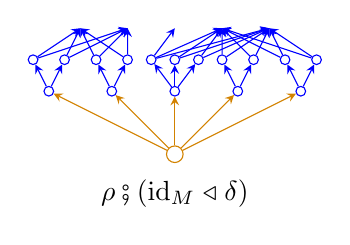
\begin{tikzpicture}
\node [ycol,vertex] (s) at (0, -8) {};
\coordinate (t1) at (-12,8) {};
\coordinate (t2) at (-6,8) {};
\coordinate (t3) at (-0,8) {};
\coordinate (t4) at (6,8) {};
\coordinate (t5) at (12,8) {};

\node [bcol,vertex,small] (m1) at (-16,0) {};
\node [bcol,vertex,small] (m2) at (-8,0) {};
\node [bcol,vertex,small] (m3) at (0,0) {};
\node [bcol,vertex,small] (m4) at (8,0) {};
\node [bcol,vertex,small] (m5) at (16,0) {};

\node [bcol,vertex,small] (m11) at (-18,4) {};
\node [bcol,vertex,small] (m12) at (-14,4) {};
\node [bcol,vertex,small] (m21) at (-10,4) {};
\node [bcol,vertex,small] (m22) at (-6,4) {};
\node [bcol,vertex,small] (m31) at (-3,4) {};
\node [bcol,vertex,small] (m32) at (0,4) {};
\node [bcol,vertex,small] (m33) at (3,4) {};
\node [bcol,vertex,small] (m41) at (6,4) {};
\node [bcol,vertex,small] (m42) at (10,4) {};
\node [bcol,vertex,small] (m51) at (14,4) {};
\node [bcol,vertex,small] (m52) at (18,4) {};

\draw [ycol,edge] (s) -- (m1);
\draw [ycol,edge] (s) -- (m2);
\draw [ycol,edge] (s) -- (m3);
\draw [ycol,edge] (s) -- (m4);
\draw [ycol,edge] (s) -- (m5);


\draw [bcol,edge] (m1) -- (m11);
\draw [bcol,edge] (m1) -- (m12);

\draw [bcol,edge] (m2) -- (m21);
\draw [bcol,edge] (m2) -- (m22);

\draw [bcol,edge] (m3) -- (m31);
\draw [bcol,edge] (m3) -- (m32);
\draw [bcol,edge] (m3) -- (m33);

\draw [bcol,edge] (m4) -- (m41);
\draw [bcol,edge] (m4) -- (m42);

\draw [bcol,edge] (m5) -- (m51);
\draw [bcol,edge] (m5) -- (m52);


\draw [bcol,edge] (m11) -- (t1);
\draw [bcol,edge] (m11) -- (t2);

\draw [bcol,edge] (m12) -- (t1);
\draw [bcol,edge] (m12) -- (t2);

\draw [bcol,edge] (m21) -- (t1);
\draw [bcol,edge] (m21) -- (t2);

\draw [bcol,edge] (m22) -- (t1);
\draw [bcol,edge] (m22) -- (t2);

\draw [bcol,edge] (m31) -- (t3);
\draw [bcol,edge] (m31) -- (t4);
\draw [bcol,edge] (m31) -- (t5);

\draw [bcol,edge] (m32) -- (t4);
\draw [bcol,edge] (m32) -- (t5);

\draw [bcol,edge] (m33) -- (t4);
\draw [bcol,edge] (m33) -- (t5);

\draw [bcol,edge] (m41) -- (t4);
\draw [bcol,edge] (m41) -- (t5);

\draw [bcol,edge] (m42) -- (t4);
\draw [bcol,edge] (m42) -- (t5);

\draw [bcol,edge] (m51) -- (t4);
\draw [bcol,edge] (m51) -- (t5);

\draw [bcol,edge] (m52) -- (t4);
\draw [bcol,edge] (m52) -- (t5);


\node at (0, -13) {$\rho \fatsemi (\id_M \sub \delta)$};
\end{tikzpicture}

  \end{center}

  Let $\cat{D}$ be the category corresponding to $D$. 
  
\end{proof}

\begin{prop}
  A polynomial left comodule amounts to a copresheaf and a presheaf on that
  copresheaf's category of elements.
\end{prop}
\begin{proof}
  Let $C$ be a polynomial comonoid and let $M$ be a left comodule on
  $C$. Denote left comodule comultiplication by $\lambda$.

  \begin{center}
    \input{fig/lmod1.tikz}
    \hspace{-.75em}
    $\underset{\lambda}{\transformto}$
    \hspace{.5em}
    \input{fig/lmod2.tikz}
  \end{center}

  \begin{center}
    \begin{tikzpicture}
\coordinate (s) at (0, -8) {};
\coordinate (t1) at (-12,8) {};
\coordinate (t2) at (-6,8) {};
\coordinate (t3) at (0,8) {};
\coordinate (t4) at (6,8) {};
\coordinate (t5) at (12,8) {};

\node [ycol,vertex,transparent] (m1) at (-15,0) {};
\node [ycol,vertex] (m2) at (-5,0) {};
\node [ycol,vertex,transparent] (m3) at (5,0) {};
\node [ycol,vertex,transparent] (m4) at (15,0) {};
\draw [dash] (s) -- (m1);
\draw [edge] (s) -- (m2);
\draw [dash] (s) -- (m3);
\draw [dash] (s) -- (m4);

\draw [ycol,edge] (m2) -- (t1);
\draw [ycol,edge] (m2) -- (t2);
\draw [ycol,edge] (m2) -- (t3);
\draw [ycol,edge] (m2) -- (t4);
\draw [ycol,edge] (m2) -- (t5);

\draw [ycol,edge,transparent,bend left=11] (m3) to (t3);
\draw [ycol,edge,transparent,bend right=11] (m3) to (t3);
\draw [ycol,edge,transparent,bend left=11] (m3) to (t4);
\draw [ycol,edge,transparent,bend right=11] (m3) to (t4);
\draw [ycol,edge,transparent,bend left=11] (m3) to (t5);
\draw [ycol,edge,transparent,bend right=11] (m3) to (t5);

\draw [ycol,transparent,edge] (m4) -- (t4);
\draw [ycol,transparent,edge] (m4) -- (t5);

\node at (0, -13) {$\lambda \fatsemi (\varepsilon \sub \id_M)$};
\end{tikzpicture}

    \quad
    $\canoniso$
    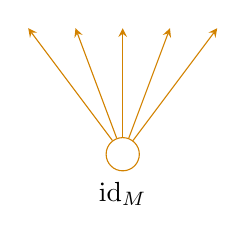
\begin{tikzpicture}
\node [ycol,vertex,large] (s) at (0, -8) {};
\coordinate (t1) at (-12,8) {};
\coordinate (t2) at (-6,8) {};
\coordinate (t3) at (0,8) {};
\coordinate (t4) at (6,8) {};
\coordinate (t5) at (12,8) {};
\draw [ycol,edge] (s) -- (t1);
\draw [ycol,edge] (s) -- (t2);
\draw [ycol,edge] (s) -- (t3);
\draw [ycol,edge] (s) -- (t4);
\draw [ycol,edge] (s) -- (t5);

\node at (0, -13) {$\id_M$};
\end{tikzpicture}

  \end{center}
  
  \begin{center}
    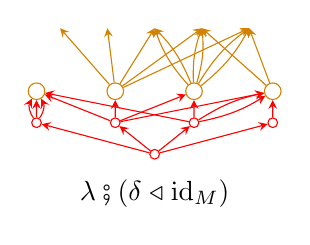
\begin{tikzpicture}
\node [rcol,vertex,small] (s) at (0, -8) {};
\coordinate (t1) at (-12,8) {};
\coordinate (t2) at (-6,8) {};
\coordinate (t3) at (0,8) {};
\coordinate (t4) at (6,8) {};
\coordinate (t5) at (12,8) {};


\node [rcol,vertex,small] (m1_) at (-15,-4) {};
\node [rcol,vertex,small] (m2_) at (-5,-4) {};
\node [rcol,vertex,small] (m3_) at (5,-4) {};
\node [rcol,vertex,small] (m4_) at (15,-4) {};

\node [ycol,vertex] (m1) at (-15,0) {};
\node [ycol,vertex] (m2) at (-5,0) {};
\node [ycol,vertex] (m3) at (5,0) {};
\node [ycol,vertex] (m4) at (15,0) {};

\draw [rcol,edge] (s) -- (m1_);
\draw [rcol,edge] (s) -- (m2_);
\draw [rcol,edge] (s) -- (m3_);
\draw [rcol,edge] (s) -- (m4_);

\draw [rcol,edge] (m1_) -- (m1);
\draw [rcol,edge,bend left=32] (m1_) to (m1);
\draw [rcol,edge,bend right=32] (m1_) to (m1);

\draw [rcol,edge] (m2_) -- (m1);
\draw [rcol,edge] (m2_) -- (m2);
\draw [rcol,edge] (m2_) -- (m3);
\draw [rcol,edge] (m2_) -- (m4);

\draw [rcol,edge] (m3_) -- (m1);
\draw [rcol,edge] (m3_) -- (m3);
\draw [rcol,edge,bend left=10] (m3_) to (m4);
\draw [rcol,edge,bend right=10] (m3_) to (m4);

\draw [rcol,edge] (m4_) -- (m4);


\draw [ycol,edge] (m2) -- (t1);
\draw [ycol,edge] (m2) -- (t2);
\draw [ycol,edge] (m2) -- (t3);
\draw [ycol,edge] (m2) -- (t4);
\draw [ycol,edge] (m2) -- (t5);

\draw [ycol,edge,bend left=11] (m3) to (t3);
\draw [ycol,edge,bend right=11] (m3) to (t3);
\draw [ycol,edge,bend left=11] (m3) to (t4);
\draw [ycol,edge,bend right=11] (m3) to (t4);
\draw [ycol,edge,bend left=11] (m3) to (t5);
\draw [ycol,edge,bend right=11] (m3) to (t5);

\draw [ycol,edge] (m4) -- (t4);
\draw [ycol,edge] (m4) -- (t5);


\node at (0, -13) {$\lambda \fatsemi (\delta \sub \id_M)$};
\end{tikzpicture}

    \quad
    $\canoniso$
    \quad
    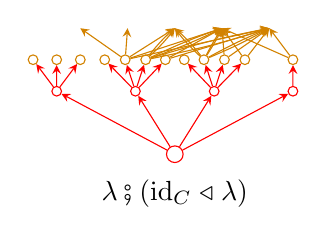
\begin{tikzpicture}
\node [rcol,vertex] (s) at (0, -8) {};
\coordinate (t1) at (-12,8) {};
\coordinate (t2) at (-6,8) {};
\coordinate (t3) at (0,8) {};
\coordinate (t4) at (6,8) {};
\coordinate (t5) at (12,8) {};

\node [ycol,vertex,small] (m11) at (-18,4) {};
\node [ycol,vertex,small] (m12) at (-15,4) {};
\node [ycol,vertex,small] (m13) at (-12,4) {};
\node [ycol,vertex,small] (m21) at (-8.9,4) {};
\node [ycol,vertex,small] (m22) at (-6.3,4) {};
\node [ycol,vertex,small] (m23) at (-3.7,4) {};
\node [ycol,vertex,small] (m24) at (-1.2,4) {};
\node [ycol,vertex,small] (m31) at (1.2,4) {};
\node [ycol,vertex,small] (m32) at (3.7,4) {};
\node [ycol,vertex,small] (m33) at (6.3,4) {};
\node [ycol,vertex,small] (m34) at (8.9,4) {};
\node [ycol,vertex,small] (m41) at (15,4) {};

\node [rcol,vertex,small] (m1) at (-15,0) {};
\node [rcol,vertex,small] (m2) at (-5,0) {};
\node [rcol,vertex,small] (m3) at (5,0) {};
\node [rcol,vertex,small] (m4) at (15,0) {};

\draw [rcol,edge] (m1) -- (m11);
\draw [rcol,edge] (m1) -- (m12);
\draw [rcol,edge] (m1) -- (m13);
\draw [rcol,edge] (m2) -- (m21);
\draw [rcol,edge] (m2) -- (m22);
\draw [rcol,edge] (m2) -- (m23);
\draw [rcol,edge] (m2) -- (m24);
\draw [rcol,edge] (m3) -- (m31);
\draw [rcol,edge] (m3) -- (m32);
\draw [rcol,edge] (m3) -- (m33);
\draw [rcol,edge] (m3) -- (m34);
\draw [rcol,edge] (m4) -- (m41);

\draw [rcol,edge] (s) -- (m1);
\draw [rcol,edge] (s) -- (m2);
\draw [rcol,edge] (s) -- (m3);
\draw [rcol,edge] (s) -- (m4);

\draw [ycol,edge] (m22) -- (t1);
\draw [ycol,edge] (m22) -- (t2);
\draw [ycol,edge] (m22) -- (t3);
\draw [ycol,edge] (m22) -- (t4);
\draw [ycol,edge] (m22) -- (t5);

\draw [ycol,edge,bend left=5] (m23) to (t3);
\draw [ycol,edge,bend right=5] (m23) to (t3);
\draw [ycol,edge,bend left=3] (m23) to (t4);
\draw [ycol,edge,bend right=3] (m23) to (t4);
\draw [ycol,edge,bend left=3] (m23) to (t5);
\draw [ycol,edge,bend right=3] (m23) to (t5);

\draw [ycol,edge] (m24) -- (t4);
\draw [ycol,edge] (m24) -- (t5);


\draw [ycol,edge,bend left=5] (m32) to (t3);
\draw [ycol,edge,bend right=5] (m32) to (t3);
\draw [ycol,edge,bend left=3] (m32) to (t4);
\draw [ycol,edge,bend right=3] (m32) to (t4);
\draw [ycol,edge,bend left=3] (m32) to (t5);
\draw [ycol,edge,bend right=3] (m32) to (t5);
\draw [ycol,edge] (m33) -- (t4);
\draw [ycol,edge] (m33) -- (t5);
\draw [ycol,edge] (m34) -- (t4);
\draw [ycol,edge] (m34) -- (t5);


\draw [ycol,edge] (m41) -- (t4);
\draw [ycol,edge] (m41) -- (t5);


\node at (0, -13) {$\lambda \fatsemi (\id_C \sub \lambda)$};
\end{tikzpicture}

  \end{center}

  Let $\cat{D}$ be the category corresponding to $D$. 
  
\end{proof}

\begin{prop}
  Polynomial bicomodules are prafunctors between presheaf categories.
\end{prop}
\begin{proof}
  Let $C$ and $D$ be polynomial comonoids and let $M$ be a bimodule
  from $C$ to $D$.  
  \begin{center}
    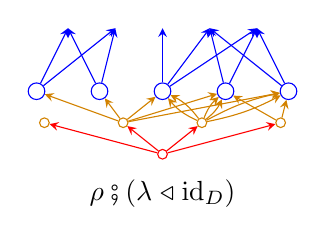
\begin{tikzpicture}
\node [rcol,vertex,small] (s) at (0, -8) {};
\coordinate (t1) at (-12,8) {};
\coordinate (t2) at (-6,8) {};
\coordinate (t3) at (-0,8) {};
\coordinate (t4) at (6,8) {};
\coordinate (t5) at (12,8) {};

\node [bcol,vertex] (m1_) at (-16,0) {};
\node [bcol,vertex] (m2_) at (-8,0) {};
\node [bcol,vertex] (m3_) at (0,0) {};
\node [bcol,vertex] (m4_) at (8,0) {};
\node [bcol,vertex] (m5_) at (16,0) {};

\node [ycol,vertex,small] (m1) at (-15,-4) {};
\node [ycol,vertex,small] (m2) at (-5,-4) {};
\node [ycol,vertex,small] (m3) at (5,-4) {};
\node [ycol,vertex,small] (m4) at (15,-4) {};

\draw [ycol,edge] (m2) -- (m1_);
\draw [ycol,edge] (m2) -- (m2_);
\draw [ycol,edge] (m2) -- (m3_);
\draw [ycol,edge] (m2) -- (m4_);
\draw [ycol,edge] (m2) -- (m5_);

\draw [ycol,edge,bend left=13] (m3) to (m3_);
\draw [ycol,edge,bend right=13] (m3) to (m3_);
\draw [ycol,edge,bend left=13] (m3) to (m4_);
\draw [ycol,edge,bend right=13] (m3) to (m4_);
\draw [ycol,edge,bend left=8] (m3) to (m5_);
\draw [ycol,edge,bend right=8] (m3) to (m5_);

\draw [ycol,edge] (m4) -- (m4_);
\draw [ycol,edge] (m4) -- (m5_);


\draw [rcol,edge] (s) -- (m1);
\draw [rcol,edge] (s) -- (m2);
\draw [rcol,edge] (s) -- (m3);
\draw [rcol,edge] (s) -- (m4);

\draw [bcol,edge] (m1_) -- (t1);
\draw [bcol,edge] (m1_) -- (t2);

\draw [bcol,edge] (m2_) -- (t1);
\draw [bcol,edge] (m2_) -- (t2);

\draw [bcol,edge] (m3_) -- (t3);
\draw [bcol,edge] (m3_) -- (t4);
\draw [bcol,edge] (m3_) -- (t5);

\draw [bcol,edge] (m4_) -- (t4);
\draw [bcol,edge] (m4_) -- (t5);

\draw [bcol,edge] (m5_) -- (t4);
\draw [bcol,edge] (m5_) -- (t5);


\node at (0, -13) {$\rho \fatsemi (\lambda \sub \id_D)$};
\end{tikzpicture}

    \quad
    $\canoniso$
    \quad
    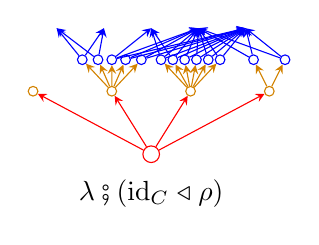
\begin{tikzpicture}
\node [rcol,vertex] (s) at (0, -8) {};
\coordinate (t1) at (-12,8) {};
\coordinate (t2) at (-6,8) {};
\coordinate (t3) at (0,8) {};
\coordinate (t4) at (6,8) {};
\coordinate (t5) at (12,8) {};

\node [ycol,vertex,small] (m1) at (-15,0) {};
\node [ycol,vertex,small] (m2) at (-5,0) {};
\node [ycol,vertex,small] (m3) at (5,0) {};
\node [ycol,vertex,small] (m4) at (15,0) {};

\node [bcol,vertex,small] (m21) at (-8.75,4) {};
\node [bcol,vertex,small] (m22) at (-6.75,4) {};
\node [bcol,vertex,small] (m23) at (-5,4) {};
\node [bcol,vertex,small] (m24) at (-3.25,4) {};
\node [bcol,vertex,small] (m25) at (-1.25,4) {};
\node [bcol,vertex,small] (m31) at (1.25,4) {};
\node [bcol,vertex,small] (m32) at (2.75,4) {};
\node [bcol,vertex,small] (m33) at (4.25,4) {};
\node [bcol,vertex,small] (m34) at (5.75,4) {};
\node [bcol,vertex,small] (m35) at (7.25,4) {};
\node [bcol,vertex,small] (m36) at (8.75,4) {};
\node [bcol,vertex,small] (m41) at (13,4) {};
\node [bcol,vertex,small] (m42) at (17,4) {};

\draw [rcol,edge] (s) -- (m1);
\draw [rcol,edge] (s) -- (m2);
\draw [rcol,edge] (s) -- (m3);
\draw [rcol,edge] (s) -- (m4);

\draw [ycol,edge] (m2) -- (m21);
\draw [ycol,edge] (m2) -- (m22);
\draw [ycol,edge] (m2) -- (m23);
\draw [ycol,edge] (m2) -- (m24);
\draw [ycol,edge] (m2) -- (m25);
\draw [ycol,edge] (m3) -- (m31);
\draw [ycol,edge] (m3) -- (m32);
\draw [ycol,edge] (m3) -- (m33);
\draw [ycol,edge] (m3) -- (m34);
\draw [ycol,edge] (m3) -- (m35);
\draw [ycol,edge] (m3) -- (m36);
\draw [ycol,edge] (m4) -- (m41);
\draw [ycol,edge] (m4) -- (m42);


\draw [bcol,edge] (m21) -- (t1);
\draw [bcol,edge] (m21) -- (t2);

\draw [bcol,edge] (m22) -- (t1);
\draw [bcol,edge] (m22) -- (t2);

\draw [bcol,edge] (m23) -- (t3);
\draw [bcol,edge] (m23) -- (t4);
\draw [bcol,edge] (m23) -- (t5);

\draw [bcol,edge] (m24) -- (t4);
\draw [bcol,edge] (m24) -- (t5);

\draw [bcol,edge] (m25) -- (t4);
\draw [bcol,edge] (m25) -- (t5);

\draw [bcol,edge] (m31) -- (t3);
\draw [bcol,edge] (m31) -- (t4);
\draw [bcol,edge] (m31) -- (t5);

\draw [bcol,edge] (m32) -- (t3);
\draw [bcol,edge] (m32) -- (t4);
\draw [bcol,edge] (m32) -- (t5);

\draw [bcol,edge] (m33) -- (t4);
\draw [bcol,edge] (m33) -- (t5);

\draw [bcol,edge] (m34) -- (t4);
\draw [bcol,edge] (m34) -- (t5);

\draw [bcol,edge] (m35) -- (t4);
\draw [bcol,edge] (m35) -- (t5);

\draw [bcol,edge] (m36) -- (t4);
\draw [bcol,edge] (m36) -- (t5);

\draw [bcol,edge] (m41) -- (t4);
\draw [bcol,edge] (m41) -- (t5);
\draw [bcol,edge] (m42) -- (t4);
\draw [bcol,edge] (m42) -- (t5);

\node at (0, -13) {$\lambda \fatsemi (\id_C \sub \rho)$};
\end{tikzpicture}

  \end{center}

  We will show that $M$ amounts to a profunctor\footnote{The notation
    $\cat{A} \prof \cat{B}$ for a profunctor
    $\cat{A}^\op \times \cat{B} \to \Set$ is due to Michael Shulman.}
  $(\int_{\cat{C}} R) \prof \cat{D}$, where $\cat{C}$ is the category
  corresponding to $C$, $\int_{\cat{C}} R$ is the category of elements
  of the copresheaf $R$ on $\cat{C}$ induced by $M$ as a left
  comodule, and $\cat{D}$ is the category corresponding to $D$.

  Such a profunctor is equivalent to a prafunctor
  $\Set^{\cat{D}} \to \Set^{\cat{C}}$. Indeed,

  \begin{align*}
    &\cong
  \end{align*}
  
\end{proof}

\begin{prop}
  Maps between bicomodules are natural transformations between prafunctors.
\end{prop}
\begin{proof}
  
\end{proof}

\begin{prop}
  Composition of bicomodules is composition of prafunctors.
\end{prop}
\begin{proof}
  Recall bicomodules from $D$ to $0$ are copresheaves on $D$ (and maps
  between such bicomodules are copresheaf maps). Hence each bicomodule
  $M$ from $D$ to $D$ induces a functor $F_M$ from $D$-copresheaves to
  $C$-copresheaves by precomposition. Accordingly, we have
  $F_{M \sub_D N} \cong F_N \fatsemi F_M$ (for bicomodules $M$
  from $C$ to $D$ and $N$ from $D$ to $E$).
  
  We show that the prafunctor corresponding to the bimodule $M$ is $F_M$. 
\end{proof}

\end{document}